% Um alles auf einmal pflegen zu können, verwenden wir \ifhtml als
% Anzeige für tex4ht oder „normales“ (PDF)LaTeX.
%
\errorcontextlines\maxdimen
\makeatletter

\newif\ifhelp\helpfalse
\newif\ifhtml\htmlfalse
%\let\ifpdf\iffalse
\newif\ifdvi\dvifalse

\def\mutabor@utput@html{
  \typeout{Producing HTML format.}
  \htmltrue
}

\def\mutabor@utput@help{%
  \mutabor@utput@html
  \typeout{Subtype: .hhp .}
  \helptrue
}

\def\mutabor@utput@latex{\typeout{Standard LaTeX output}}

\providecommand\outputformat{latex}
\@ifundefined{mutabor@utput@\outputformat}{
  \typeout{Undefined output format%
    \@ifundefined{outputformat}{}{ \outputformat}.
  }
}{
  \csname mutabor@utput@\outputformat\endcsname
}

%\def\htmltrue{\let\ifhtml\iftrue}
%\def\htmlfalse{\let\ifhtml\iffalse}
%\ifx\ifhtml\undefined
%  \htmlfalse
%\else
%  \htmltrue
%\fi
% 
% Ein Kommentar aus dem alten Handbuch... ;-)
%
% =====================================================
%
% NOCH ZU KORRIGIEREN :
%
%
% - oberflächenspezifische Beschreibungen auslagern !
%
% =====================================================
%
% Koma-Skript liefert ein paar nützliche zusätzliche Definitionen
%

\documentclass[a4paper,BCOR1.0cm]{scrbook}
%
% Für tex4ht müssen wir auch tex4ht laden...
\ifhtml
\input htmlpreamble.tex
\fi
% Einstellungen für Latex laden
\usepackage[utf8]{inputenc}
\usepackage[T1]{fontenc}
\usepackage{babel}
% Some mathematics
\usepackage{amsmath}
% Exteren Referenzen und Hyperref laden. 
% Das kann unterschiedlich ablaufen.
\ifhtml
 %  \Configure{html}{html.de}
  \ifpdfoutput{\pdfoutput0\relax}{}
   \usepackage{xr-hyper}
   \usepackage{hyperref}
\else
 %  \usepackage{mathpazo}
  \usepackage{xr-hyper}
  \usepackage[extension=pdf]{hyperref}
\fi
% Überschriften als Referenzen einfügen.
\usepackage{nameref}
%\usepackage{zref-xr}
%\zxrsetup{toltxlabel}
\usepackage{graphicx}
\usepackage{tikz}
\usepackage{listings}
\usepackage{listingsutf8}

\lstdefinelanguage{Mutabor}{%
%otherkeywords={:,=,:=,+,-,*,\(,\),[,],.,\,,;},
%morekeywords=[1]{},%
%Befehle
morekeywords=[1]{INTERVALL,TON,TONSYSTEM,UMSTIMMUNG,HARMONIE,LOGIK,%
INTERVAL,TONE,TONESYSTEM,RETUNING,PATTERN,LOGIC,SHIFTED},%
%Funktionen
morekeywords=[2]{MIDIKANAL,WURZEL,TASTE,MIDIIN,MIDIOUT,ANSONSTEN,%
FORM,ROOT,MIDICHANNEL,KEY,ELSE},
%morekeywords=[3]{=,-},
%Datentypen
%morekeywords=[4]{},%
   sensitive=false,%
   %alsoletter={=,-},
%   alsoletter={+,-,*,/,.,:,=,<,>}, %(,),[,],.,\,,:,;,^,@,
%   morecomment=[s]{(*}{*)},%
%   morecomment=[s]{\{}{\}},%
%   morecomment=[l]{//},%
   morecomment=[s]{"}{"},%
%   moredelim=*[s]{\[}{\]},%
%   moredelim=*[s]{(}{)}
%   moredelim=*[s]{\{}{\}}
%   morestring=[d]'%
  }%[keywords,comments,strings]%

\lstloadlanguages{Mutabor}
\lstset{%
  tabsize=8,
  language=Mutabor,
  defaultdialect=Mutabor,
  basicstyle=\ttfamily\color[rgb]{0.5,0,0},
  identifierstyle=\color{black},
  keywordstyle=[1]{\color[rgb]{0,0.5,0}\bfseries},
  keywordstyle=[2]{\color[rgb]{0,0,0.5}\bfseries},
  keywordstyle=[4]{\color{black}},
  keywordstyle=[3]{\color[rgb]{0.5,0,0}},
  stringstyle=\color{blue},
  commentstyle=\color[rgb]{0.5,0.5,0.5}\textit,
  inputencoding=utf8,
  extendedchars=false,
  showtabs=false,
  showspaces=false,%
  texcl=true,%
  escapechar=",
  escapebegin={\color[rgb]{0.5,0.5,0.5}\expandafter\textit\bgroup%
    \obeylines\obeyspaces
    \dq},
  escapeend={\dq\egroup}
}

%%% Local Variables: 
%%% mode: latex
%%% TeX-master: t
%%% End: 

%
% Das Handbuch wurde mit emTeX geschrieben. TeTeX versteht die emTeX
% specials. Also verwenden wir sie.
\usepackage{tsemlines}
% Makeindex laden
\usepackage{makeidx}
%
% file: macht uns die relativen Links kaputt :-(
%
\hyperlinkfileprefix{}
%
% Kolumnentitel erleichtern dem Leser die Orientierung
%
\AtBeginDocument{\pagestyle{headings}}
% 
% Titelei
\setkomafont{title}{\fontfamily{\rmdefault}\fontseries{bx}\huge}
\title{\rmfamily\texorpdfstring{\mutabor\\[\baselineskip]}{MUTABOR --}
 \LARGE\slshape Ein computergesteuertes Musikinstrument \\
	  zum Experimentieren mit\\
	  Stimmungslogiken und Mikrotönen}
\author{Volker Abel, Peter Reiss,\\ Rüdiger Krauße und Tobias Schlemmer}
\date{Programmversion $3.0x$ (\the\year)}
\ifhtml\else
  \publishers{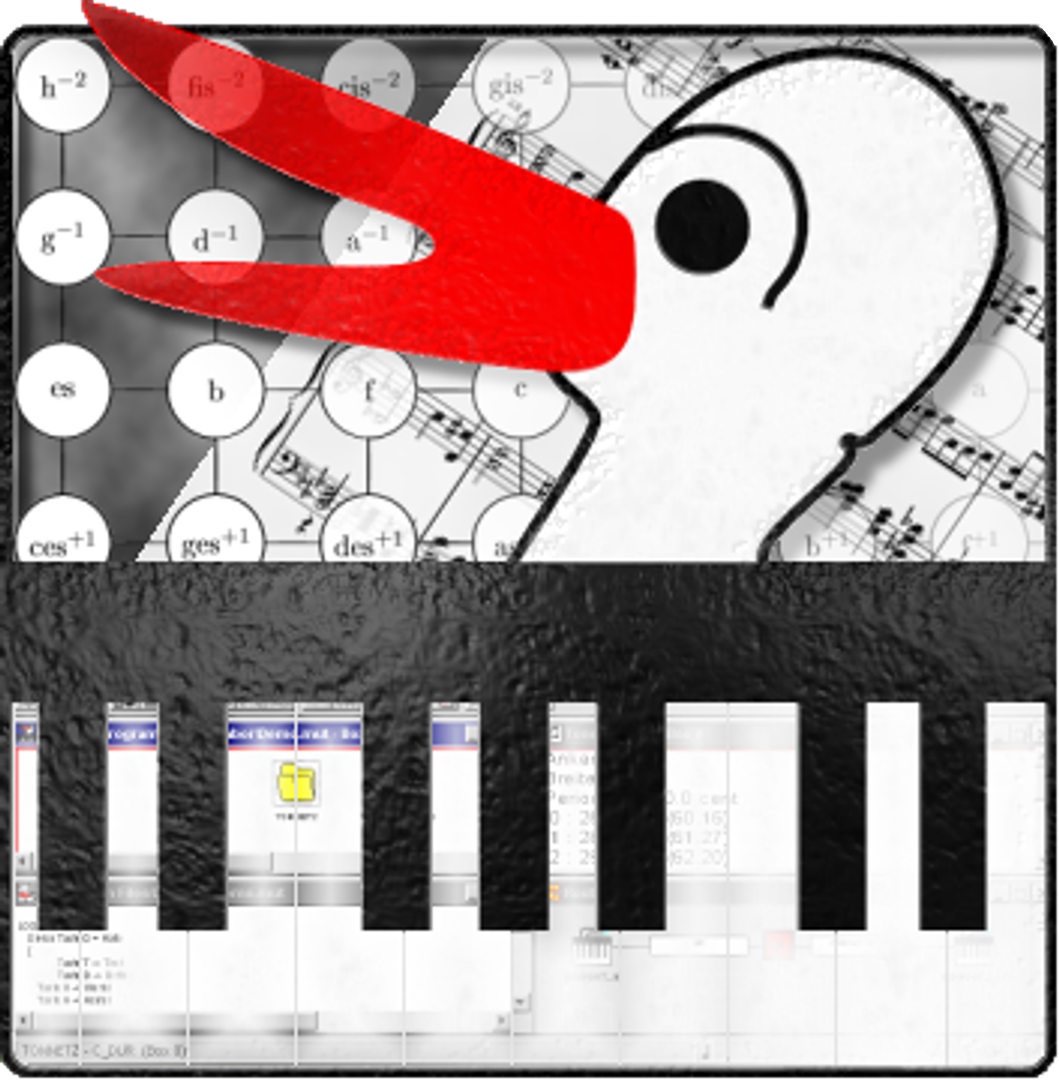
\includegraphics[width=0.5\linewidth]{Mutabor-Logo}}
\fi
\lowertitleback{\footnotesize\copyright 1991, 1992 Volker Abel \& Peter Reiss\\
\copyright 2006–\the\year TU Dresden, Institut für Algebra}
%
% Index-Datei öffnen
%
\makeindex
\hyphenation{wei-te-re Ton-sys-tem Ton-sys-te-me}
%\parindent 0mm
%\parskip 5pt
%\textheight 18.5cm
%
% Jetzt wirds ein wenig wüst.
%
% Wir wollen mit wenig Aufwand die Labels auch für Hyperlinks
% verwenden. Damit sparen wir uns zusätzliche Anker.
% 
\makeatletter
%
% \XR@ext enthält die Erweiterung für Querverweise. Wenn wir auf
% Buchanfänge usw. verweisen wollen, kann uns xr-hyper nicht
% undbedingt helfen. (oder wir müsste das entsprechend definieren).
% Einfacher ist es wohl, wir nehmen den Dateinamen.
%
\newcommand\makefilename[1]{#1.\XR@ext}
%
%
% erstes von sechs Argumenten wiedergeben und Rest verwerfen
\def\ts@firstofsix#1#2#3#4#5#6{#1}
%
\ifhtml
% voreinstellungen, um „:“ als Buchstaben zu behandeln (für tex4ht)
% 
% Herausfiltern des Verlinkungsmakros aus Querverweis-Speichern
%
\def\ts@parse@ref@a#1#2\ts@end@parse{\ts@parse@ref@b#1\ts@end@parse}
\def\ts@parse@ref@b#1#2#3\ts@end@parse{#1{#2}}
%
% Setzen des Verweises.
% Das erste Argument mus zunächst expandiert werden, bevor es
% überhaupt mit den obigen makros geparst werden kann. Wir sichern uns
% das ganze in einem temporären Makro zusammen mit dem Ankertext. 
%
\def\ts@setref#1#2#3{%
  \expandafter\expandafter
  \expandafter\def
  \expandafter\expandafter
  \expandafter\ts@@tmp
  \expandafter\expandafter
  \expandafter{%
    \expandafter\ts@parse@ref@a#1\ts@end@parse{#2}}%
%
% Wir hacken uns in \@setref hineein.
% dort steht: \expandafter #2#1. Wir liefern aber alles, was wir
% brauchen schon in #2 mit, verwerfen also alles aus #1.
% wir machen daraus \expandafter\ts@firstofsix\expandafter\ts@@tmp#1
% damit wird zunächst #1 expandiert und dann verworfen.
% Genial nicht ;-)?
%
% Alternativ könnte man auch mit \@firstoftwo arbeiten. Hier muss man
% aufpassen, dass das erste Argument nicht falsch expandiert wird.
% \setref#1{\@firstoftwo{\ts@@tmp}}{#3}
%
  \@setref#1{% 
    \ts@firstofsix%
      \expandafter\ts@@tmp}{#3}%
}
%
% Jetzt können wir das eigentliche Linkmakro definieren. 
%
% Wenn die Referenz nicht definiert ist, setzen wir den Ankertext und
% rufen setref auf, damit die entsprechende Warnung ausgespuckt
% wird. Die ausgegebenen Fragezeichen setzen wir in weißer Farbe in
% eine 0pt breite Box (llap). Damit kommt es nur zu minimalen
% Verschiebungen (Kerning) zwischen undefiniert und definiert. 
%
% Ist die Referenz definiert, wird sie verwendet, um einen Link zu erzeugen.
\newcommand\ts@reflink[2]{%
  \@ifundefined{r@#1}{%
    \textcolor{red}{%
      #2%
      \color{white}{%
        \llap{%
          \@safe@activestrue
          \edef \RefArg {#1}
          \expandafter\ts@setref\csname r@#1\endcsname{{\@safe@activesfalse #2}}{#1}%
          \@safe@activesfalse
        }%
      }%
    }%
  }{%
    \@safe@activestrue
%    \let\::ref \T:ref
    \expandafter\ts@setref\csname r@#1\endcsname{{\@safe@activesfalse #2}}{#1}%
%    \def\::ref{\protect\T@ref}%
    \@safe@activesfalse
  }%
}
% : wiederherstellen
%\ts@savecatcode
\else
% Hier läuft es eigentlich genauso ab, wie bei der
% tex4ht-Variante. Nur werden jetzt die Verweise etwas anders kodiert,
% so dass man sie nicht wirklich neu parsen muss.
\newcommand\ts@reflink[2]{%
\begingroup%\tracingall
  \def\ts@tmp{{\@safe@activesfalse #2}}%
  \@ifundefined{r@#1}{%
    \textcolor{red}{%
      #2%
      \color{white}{%
        \llap{%
          \@safe@activestrue
          \expandafter\@setref\csname r@#1\endcsname{\ts@firstofsix\ts@tmp}{#1}%
          \@safe@activesfalse
        }%
      }%
    }%
  }{%
    \@safe@activestrue
    \expandafter\@setref\csname r@#1\endcsname{\ts@firstofsix\ts@tmp}{#1}%
    \@safe@activesfalse
  }%
%\show\ts@reflink
\endgroup
}
\fi
%\newcommand\ts@@reflink{\protect\ts@reflink}
%
% die anderen definierten Referenz-Makros sind auch \protect-et
% definiert. Also machen wir das auch mit einem Querverweis auf ein
% Label mit einem beliebigen Ankertext.
%
\newcommand\reflink{\protect\ts@reflink}
%
% Referenz durch Titel, ggf. Zusatz (wie z.\,B. Buchname bei externen
% Referenzen) und Seite bei nicht-HTML-Ausgabe. Der Zusatz wird in []
% angegeben. Das erledigen wir durch zwei Makros:
%
\newcommand\tsciteref[1]{%
  \frqq\nameref{#1}\flqq
  \@ifnextchar[{\ts@cite@ref{#1}}{\ts@cite@@ref{#1}}
}
% mit optionalem Argument: Leerzeichen+Zwischentext und dann
% Seitenangabe ohne zweites Arg.
\def\ts@cite@ref#1[#2]{ #2\ts@cite@@ref{#1}}
% Ohne optionales Argument: Seitenangabe
\def\ts@cite@@ref#1{%
  \ifhtml\else{}
  auf Seite \pageref{#1}%
  \fi
}
% So ziemlich alles, was man referenzieren kann:
% Verweis-Typ: Kapitel, Abschnitt usw. 
% Nummer, Titel, ggf. optionales Argument, ggf. Seite.
% Syntax \vollref{Label}[zwischentext] (letzteres wird durch
% \tsciteref eingeführt
\newcommand\vollref[1]{\autoref{#1} \tsciteref{#1}}
%
% a try to generate file names from titles
%
\newcommand\helpsection[2]{% 1 file name, 2 label for hhk
        \@ifundefined{mut@b@r@file@\string#1}{%
                \xdef\mut@bor@nextfile{\string#1}%
		\expandafter\def\csname mut@b@r@file@\string#1 \endcsname{}
        }{
                \PackageError{mutabor.cfg}{Filenaeme \dq#1\dq already used.}%
        }%
        \@ifundefined{mut@b@r@label@\string#1}{%
		\expandafter\def\csname mut@b@r@label@\string#1 \endcsname{}
                %\set label for section.
        }{
                \PackageError{mutabor.cfg}{Help label \dq#1\dq already defined.}%
        }%
}
%
% Und hier sind wir aus den Interna heraus.
%
\makeatother
%
% Ein Makro zur vereinfachten Umwandlung der Mutabor-Hilfe mit Querverweisen.
%
\newcommand\tsreflink[2]{\reflink{sec:#2}{#1}}
%
% Der Name unseres Programmes
%
\newcommand\mutabor[1][]{\texorpdfstring{\textsc{Mutabor#1}}{MUTABOR#1}}
%
% Vorbereitung zur Verwendung des Pakets keystroke. Damit werden
% Tasten als Piktogramme angezeigt.
%
\usepackage{keystroke}%
%\providecommand\keystroke[1]{#1}
%
% Schlüsselworte und sonstiger Quelltext in Schreibmaschinenschrift.
%
\newcommand\keyword[1]{\texttt{#1}}
%
% Wir wollen die Handbücher ja nicht nur in die CD integrieren.
%
\ifhtml
  \newcommand\cdoronline[2]{#1}
\else
  \newcommand\cdoronline[2]{#2}
\fi

\newcommand\sourcecode{\texttt}%
\newcommand\filename{\texttt}

\newcommand\mutimage[2]{%
  \ifhtml
  \Picture{#1}%
  \else
  \includegraphics#2
  \fi
}

\newcommand\translate[1]{\textcolor{red}{#1}}
\newcommand\textat{@}
\newcommand\textapostrophe{'}

% define some names:
\AtBeginDocument{%
	\providecommand\addchapname{\chaptername}%
	\providecommand\likesectionname{\sectionname}%
}
\endinput


